\documentclass[]{article}
\usepackage{lmodern}
\usepackage{amssymb,amsmath}
\usepackage{ifxetex,ifluatex}
\usepackage{fixltx2e} % provides \textsubscript
\ifnum 0\ifxetex 1\fi\ifluatex 1\fi=0 % if pdftex
  \usepackage[T1]{fontenc}
  \usepackage[utf8]{inputenc}
\else % if luatex or xelatex
  \ifxetex
    \usepackage{mathspec}
  \else
    \usepackage{fontspec}
  \fi
  \defaultfontfeatures{Ligatures=TeX,Scale=MatchLowercase}
\fi
% use upquote if available, for straight quotes in verbatim environments
\IfFileExists{upquote.sty}{\usepackage{upquote}}{}
% use microtype if available
\IfFileExists{microtype.sty}{%
\usepackage{microtype}
\UseMicrotypeSet[protrusion]{basicmath} % disable protrusion for tt fonts
}{}
\usepackage{hyperref}
\hypersetup{unicode=true,
            pdfborder={0 0 0},
            breaklinks=true}
\urlstyle{same}  % don't use monospace font for urls
\usepackage{graphicx,grffile}
\makeatletter
\def\maxwidth{\ifdim\Gin@nat@width>\linewidth\linewidth\else\Gin@nat@width\fi}
\def\maxheight{\ifdim\Gin@nat@height>\textheight\textheight\else\Gin@nat@height\fi}
\makeatother
% Scale images if necessary, so that they will not overflow the page
% margins by default, and it is still possible to overwrite the defaults
% using explicit options in \includegraphics[width, height, ...]{}
\setkeys{Gin}{width=\maxwidth,height=\maxheight,keepaspectratio}
\IfFileExists{parskip.sty}{%
\usepackage{parskip}
}{% else
\setlength{\parindent}{0pt}
\setlength{\parskip}{6pt plus 2pt minus 1pt}
}
\setlength{\emergencystretch}{3em}  % prevent overfull lines
\providecommand{\tightlist}{%
  \setlength{\itemsep}{0pt}\setlength{\parskip}{0pt}}
\setcounter{secnumdepth}{0}
% Redefines (sub)paragraphs to behave more like sections
\ifx\paragraph\undefined\else
\let\oldparagraph\paragraph
\renewcommand{\paragraph}[1]{\oldparagraph{#1}\mbox{}}
\fi
\ifx\subparagraph\undefined\else
\let\oldsubparagraph\subparagraph
\renewcommand{\subparagraph}[1]{\oldsubparagraph{#1}\mbox{}}
\fi

\date{}

\begin{document}

\section{GeneticsInspiredNeuralNetworkTuning}\label{geneticsinspiredneuralnetworktuning}

\subsection{Introduction:}\label{introduction}

The first analysis for optimizing neural network is done using
evolutionary genetics. Search space consists of 5 hyper-parameters:
activation functions, optimizers, hidden layers, nodes in hidden layers
and dropout.

Seven activation functions included are: sigmoid, elu, selu, relu, tanh,
hard\_sigmoid, linear. In addition to this, optimizers include sgd,
rmsprop, adagrad, adadelta, adam, adamax, nadam. Hidden layers range
from 1-20. Nodes/neurons range from 32-1024. Dropouts range from 0.1 to
0.5.

Using genetic algorithm, the networks are initialized using random sets
of configuration variables. These networks then exchange
hyper-parameters with each others(a.k.a. crossover). The networks get
the change to mutate @2\%. This process is called as breeding. The
process repeats for generations. Due to memory and time constraints, the
whole code ran for 1day-5hours, fetching results for 10 generations.

Number of networks initialized = 7 Processors used = 1

\subsection{Requirements:}\label{requirements}

\begin{enumerate}
\def\labelenumi{\arabic{enumi}.}
\tightlist
\item
  Server: Scientific Linux release 7.5 (Nitrogen)
\item
  conda 4.5.10
\item
  Python 2.7.15 :: Anaconda, Inc.
\item
  numpy 1.15.0
\item
  Keras 2.2.2
\item
  Tensorflow 1.5
\item
  gcc: gcc (GCC) 4.8.5 20150623 (Red Hat 4.8.5-28)
\item
  ld: ldd (GNU libc) 2.17
\end{enumerate}

\subsection{Usage:}\label{usage}

\begin{verbatim}
python snnt.py
\end{verbatim}

This saves the output in a log file.

A quick crossstab of the tested combinations of hyper-parameters is
shown below. It can be easily seen that while evaluating hyper-parameter
combinations for training out of 7 activation functions, hard\_sigmoid
and elu couldn't come in any set of combinations for the 7 networks, in
any of the 10 generations. 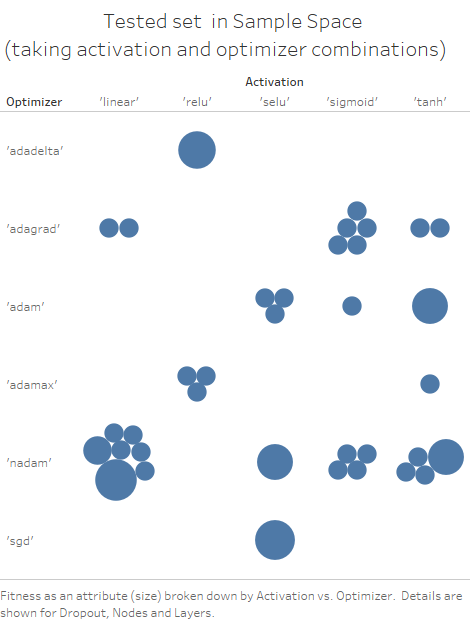
\includegraphics{./Images/Samples.png}

A more detailed plot is as follows. The size of the bubbles denote the
fitness. While with linear activation function, `nadam' optimizer has
been more frequently tested, with sigmoid activation function, adagrad
is more frequently tested. 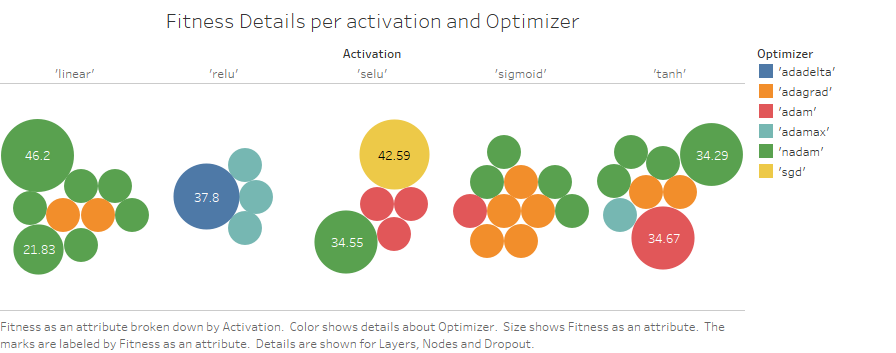
\includegraphics{./Images/Details.png}

A time lapse of various generations at network level is shown below.
Since, it's a sequential code, the graphs can be seen in a beautiful
stair-case format. Total time taken is \textasciitilde{}29 hours for 10
generations. Since tensorflow saves the previous model data, the time
taken increases with generation with 1st generation taking 139 minutes
and going as high as 200 minutes in later generations.
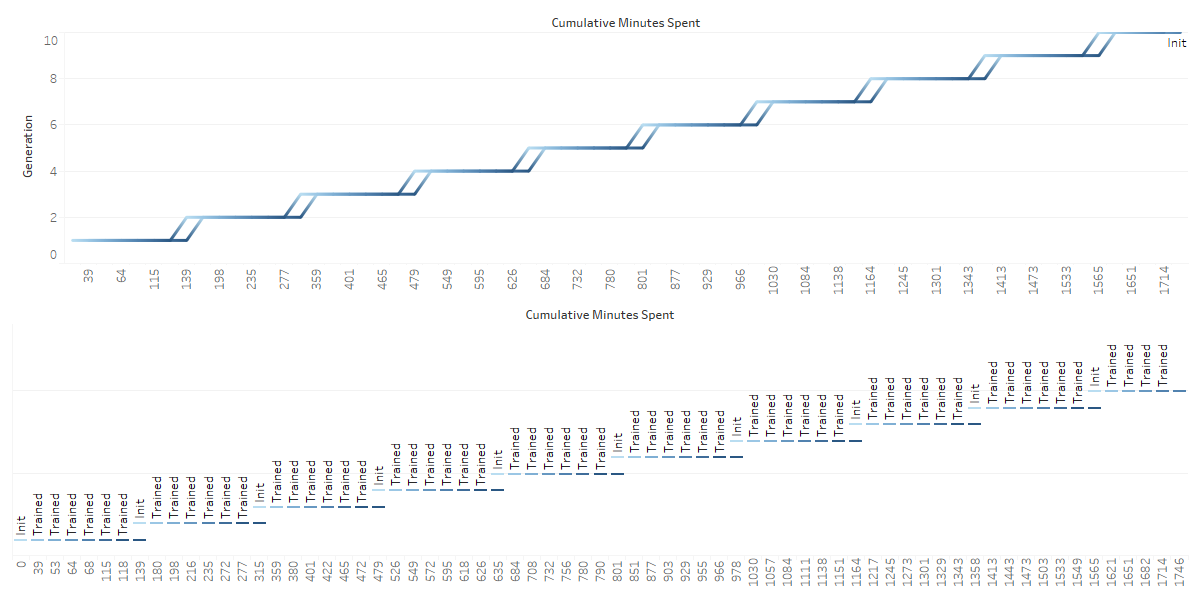
\includegraphics{./Images/TimeDashboard.png}
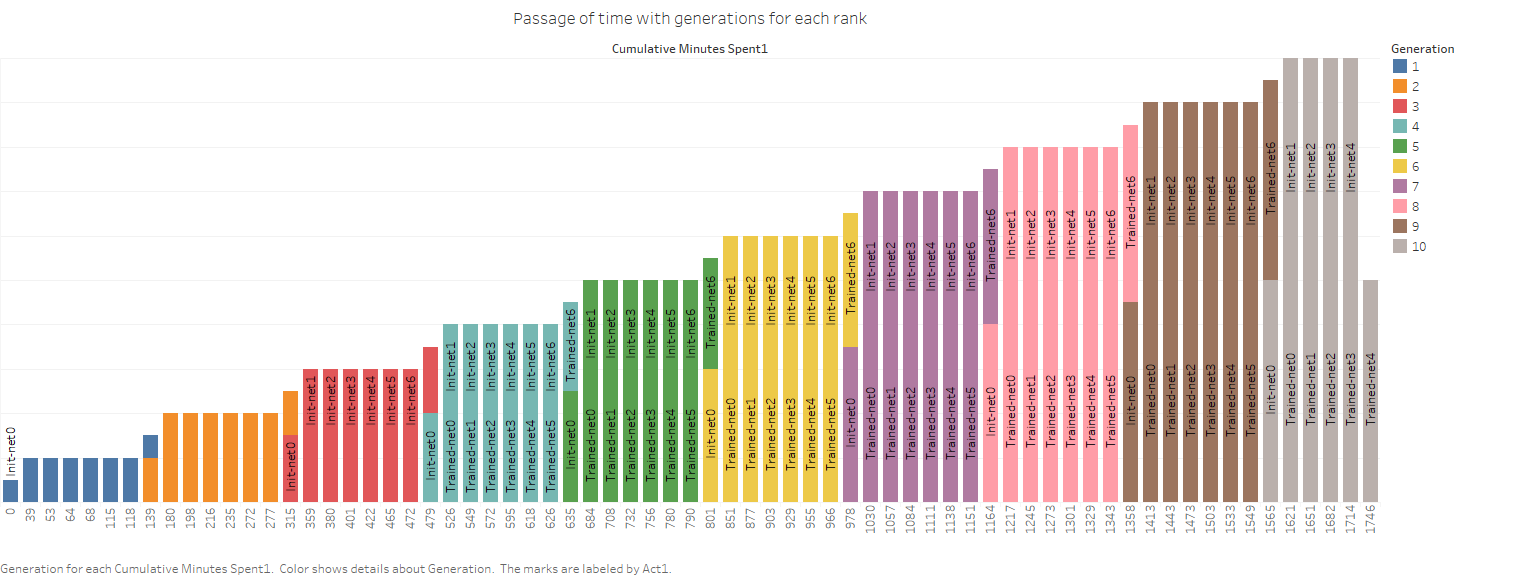
\includegraphics{./Images/PassageTime.png}

Since, initialization of hyper-parameters is random and total possible
combinations of hyper-parameters is tens of thousands, it is highly
unlikely to get the best combination initialized of bred. To check this,
a population of 70 networks is initialized on one processor. The code
ran for 2days(time limit of TCHPC-Boyle cluster), running only for 1
generation(70 networks trained) and training 28 networks of the second
generation.

A snippet of change in fitness with networks: * in the first case with
initialization of 7 networks and * second case where 70 networks are
initialized is as follows: 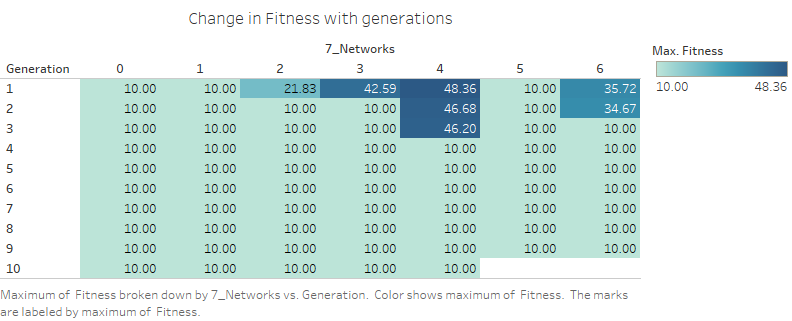
\includegraphics{./Images/7Ranks.png}
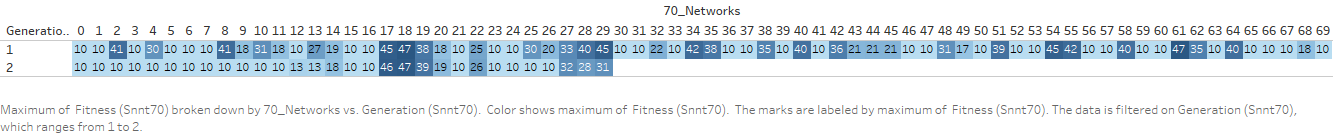
\includegraphics{./Images/70Ranks.png}

The following fitness - heatmap shows fitness variation with generations
and networks. The crosstab of activation functions and optimizer
functions uses colored cells to display the level of fitness for various
combinations. The cell text has number of hidden layers, nodes, dropout
and fitness respectively. The below graphs are for 7 and 70 networks
initialized cases respectively, where only the best hyper-parameter
configurations (\emph{as per activation and optimizer}) are shown. In 7
networks case, `sgd' optimizer has been tested once with `selu' and
showed best accuracy of 48.4\%. Linear activation function showed good
accuracy with `nadam' when the number of nodes are 1024 in 3 hidden
layers. 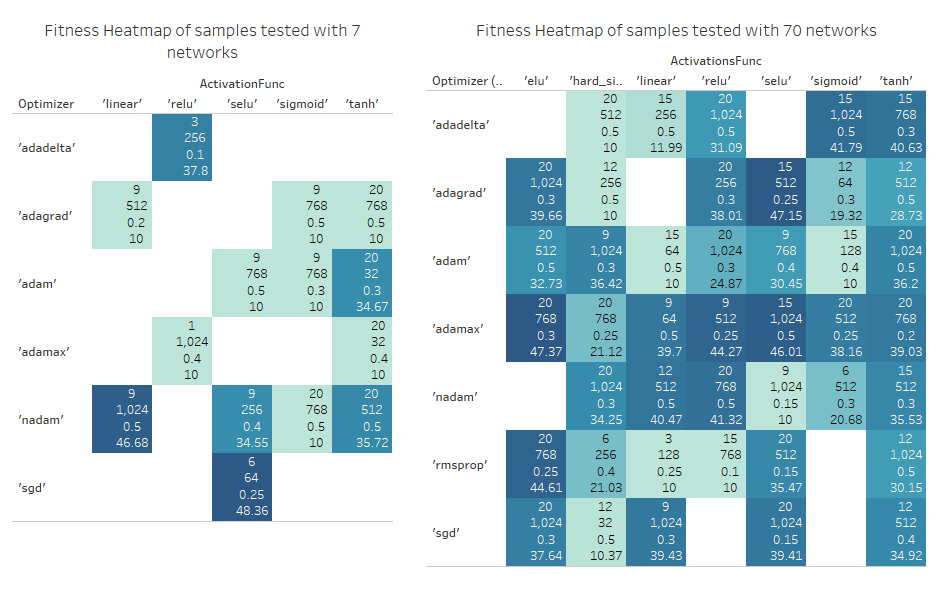
\includegraphics{./Images/HeatMap.png}

Looking at the 70 networks heatmap, it can be concluded that most of the
combinations of activation functions and optimizer functions have been
tried. The best accuracy achieved is using selu-adagrad-15 layers-512
nodes-0.25 dropout

\end{document}
